%\documentclass[10pt]{beamer}
\documentclass[10pt,handout]{beamer}
\usepackage[spanish]{babel}
% % \usepackage[backend=biber, style=authoryear-icomp]{biblatex}
\resetcounteronoverlays{exx}
\usepackage{mdframed}
\usepackage{tikz}
\usepackage{blindtext}
\usepackage{tipa}
% \usepackage{cgloss4e}
% \usepackage{gb4e}
% \usepackage{qtree}
\usepackage{cancel}
\usepackage{wrapfig}
\usepackage{soul}
\usepackage{enumerate}
\usepackage{longtable}
\graphicspath{ {./figures/} } % declaramos donde estan las imagenes
\usepackage[labelformat=simple]{subcaption} % para varias imagenes juntas
\renewcommand\thesubfigure{(\alph{subfigure})}
\usepackage[utf8]{inputenc}
\usepackage{amsmath}
\usepackage{amsfonts} % simbolos como el I de matriz identidad
\usepackage{bm}
\usepackage{graphicx} % paquete para ver imagenes
\usepackage{setspace}
\usepackage[T1]{fontenc}
\usepackage{parskip}
\usepackage{color}
\usepackage{framed}

\usetheme{Copenhagen}
\definecolor{frenchblue}{rgb}{0.0, 0.45, 0.73} % ESTE!!!!

\setbeamercolor{block body}{bg=frenchblue!50}
\setbeamercolor*{structure}{fg=frenchblue,bg=blue}
\setbeamercolor{normal text}{fg=black}
\setbeamercolor{frametitle}{bg=black}
\setbeamertemplate{frametitle}[default][center]
\setlength{\parskip}{12pt}
\useoutertheme{infolines} % me comia mucho espacio de la otra fgorma
\makeatother
\setbeamertemplate{footline}
{
  \leavevmode%
  \hbox{%
  \begin{beamercolorbox}[wd=.3\paperwidth,ht=2.25ex,dp=1ex,center]{author in head/foot}%
    \usebeamerfont{author in head/foot}\insertshortauthor
  \end{beamercolorbox}%
  \begin{beamercolorbox}[wd=.6\paperwidth,ht=2.25ex,dp=1ex,center]{title in head/foot}%
    \usebeamerfont{title in head/foot}\insertshorttitle
  \end{beamercolorbox}%
  \begin{beamercolorbox}[wd=.1\paperwidth,ht=2.25ex,dp=1ex,center]{date in head/foot}%
    \insertframenumber{} / \inserttotalframenumber\hspace*{1ex}
  \end{beamercolorbox}}%
  \vskip0pt%
}
\makeatletter
\setbeamertemplate{navigation symbols}{}
%\setbeameroption{show notes}
\setbeameroption{hide notes}


\usepackage{hyperref}

\title[Algoritmos y estructuras de datos 2]{Oblivious Data Structures}
\author[Matias Mazzanti]{Matias Mazzanti}


\institute{DC-UBA}
\date{01 de Agosto de 2022}

\titlegraphic{
\includegraphics[,height=2cm,keepaspectratio]{logo.pdf}     }
%\logo{
\includegraphics[height=2.5cm]{logo.PDF}}

\begin{document}

\begin{frame}

\maketitle

\end{frame}
\section{}
\begin{frame}
\frametitle{Introducción}
\begin{mdframed}[backgroundcolor=frenchblue!20]
 Veremos paper de Daniele Micciancio: Oblivious Data Structures: Applications to Cryptography
\end{mdframed}
\begin{itemize}\itemsep-1em
   \item Introducción.
     \vspace{-0.3cm}
  \begin{itemize}\itemsep-1em
     \item Definiciones Criptografía.
      \item Firma digital.
      \item Problemas de privacidad.
      \item Repaso arboles.
  \end{itemize}
\item Estructura de datos.
     \vspace{-0.3cm}
  \begin{itemize}\itemsep-1em
      \item Nueva estructura de datos.
      \item Algoritmos.
  \end{itemize}
  \item Demostración
     \vspace{-0.3cm}
  \begin{itemize}\itemsep-1em
     \item Complejidad.
    \item Distribución de probabilidades.
  \end{itemize}
    \item Conclusiones.
\end{itemize}
\end{frame}
\section{Introducción}
\begin{frame}
\frametitle{Definiciones}
\textbf{Criptografía}: Codificar mensajes y operaciones por motivos de seguridad.

\pause
\textbf{Firma digital}: mecanismo de criptográfico. Permite corroborar que un documento sea el correcto.
En general esquema de clave publica. Encripto con clave secreta, usuarios decriptan con clave publica.
\pause

\textbf{Firma digital incremental}: Al modificar el documento, incremento la
firma sin necesidad de hacer una firma nueva.

\pause
Ejemplo:
\begin{itemize}
  \item Enviar un documento a multiples usuarios: firmo una única vez el documento
    y modifico de forma incremental por cada usuario.
\pause
  \item Cámara de vigilancia: envía frecuentemente imágenes firmadas en periodos cortos de tiempo.
        Como posiblemente el cambio entre cuadro a cuadro es chico y hay poco tiempo, hago firma incremental.
\end{itemize}

\end{frame}

%%%%%%%%%%%%%%%%%%%%%%%%%%%%%%%%%%%%%%%%%%%%%%%%%%%%%%%%%%%%%%%%%%%%%%%%%%%%%%%%%%%%%%%%%%%%%%%%%%%%
\begin{frame}
\frametitle{Problemas de Firma digital incremental}

Dos problemas fundamentales: Seguridad y privacidad.

\pause
\textbf{Seguridad}:

Un adversario puede conseguir un documento firmado (sin la clave) y no tiene que ser posible
que produzca una modificación en el documento, volver a firmar y que no se note.

\pause
\textbf{Privacidad}:

Una firma digital generado por un algoritmo de firma incremental no solo depende del documento
$D$ si no de las operaciones que se le hicieron.
Cierta información de como se  obtuvo $D$ como secuencia de operaciones de edición podrían ser
calculadas con la firma del documento final.
\end{frame}
%%%%%%%%%%%%%%%%%%%%%%%%%%%%%%%%%%%%%%%%%%%%%%%%%%%%%%%%%%%%%%%%%%%%%%%%%%%%%%%%%%%%%%%%%%%%%%%%%%%%%%%%%%%%%%%

\begin{frame}
\frametitle{Firma digital incremental}

\textbf{Esquema básico}: Firmo de forma no incremental el documento con la modificación junto con su firma pasada.
El tiempo de esto es proporcional al cambio realzado y no al documento entero.

\begin{figure}[h!]
    \centering
    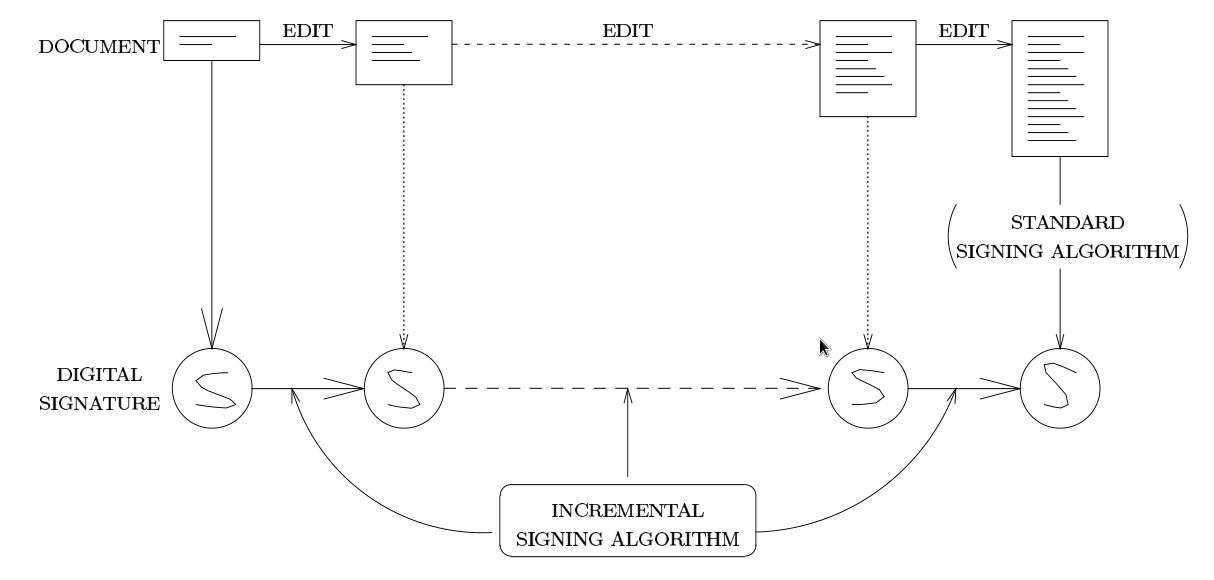
\includegraphics[scale=0.25]{firma.jpg}
\end{figure}


\end{frame}

%%%%%%%%%%%%%%%%%%%%%%%%%%%%%%%%%%%%%%%%%%%%%%%%%%%%%%%%%%%%%%%%%%%%%%%%%%%%%%%%%%%%%%%%%%%%%%%%%%%%%%%%%%%%%%%

\begin{frame}
\frametitle{Firma digital incremental}

Primera propuesta Bellare, Goldreich y Goldwasser:
\begin{itemize}\itemsep-1em
  \item El documento se divide en bloques y a cada uno se le pone una firma digital convencional.
\pause
\item Estructura de datos: árbol 2-3 para mantener el árbol balanceado.
  \item  Cada resultado de estos es una hoja del árbol de búsqueda.
\pause
  \item Los nodos internos son etiquetados con una firma digital de sus hijos y un entero contando
la cantidad de hojas del sub árbol, que tiene de raíz a dicho nodo.
\item Por cada operación básica, la firma del documento es actualizada usando los Algoritmos
de los arboles 2-3 y recomputando las firmas de los nodos internos que fueron modificados.
Operaciones en tiempo O(logn).
\end{itemize}


\pause
Si el algoritmo de firma no incremental es seguro también lo sera el incremental.

\end{frame}

%%%%%%%%%%%%%%%%%%%%%%%%%%%%%%%%%%%%%%%%%%%%%%%%%%%%%%%%%%%%%%%%%%%%%%%%%%%%%%%%%%%%%%%%%%%%%%%%%%%%%%%%%%%%%%%


\begin{frame}
\frametitle{Privacidad}
\textbf{Problema}: No tiene privacidad. Cada actualización contiene información de las
modificaciones realizadas.
\vspace{-0.2cm}
\begin{itemize}\itemsep-1em
  \item Si tenemos el árbol ABCE e insertamos D obtenemos la figura $a$.
  \item Si tenemos el árbol ACDE e insertamos B obtenemos la figura $b$.
\end{itemize}

\begin{figure}[h!]
    \centering
    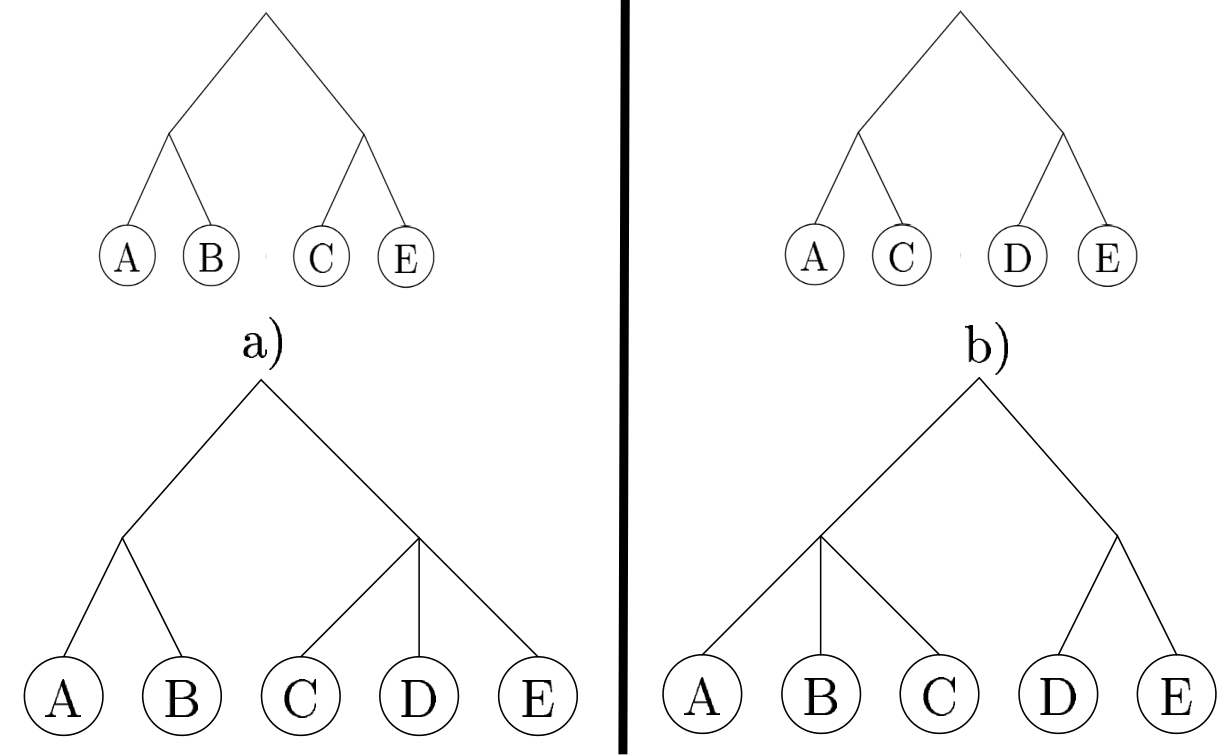
\includegraphics[scale=0.25]{2-3tree.jpg}
\end{figure}

\pause
La estructura del árbol me da información del orden de los nodos insertados.
En caso que no lo de llamaremos a esa propiedad \texttt{obliviousness} (\textbf{inadvertida}).

\end{frame}
%%%%%%%%%%%%%%%%%%%%%%%%%%%%%%%%%%%%%%%%%%%%%%%%%%%%%%%%%%%%%%%%%%%%%%%%%%%%%%%%%%%%%%%%%%%%%%%%%%%%

\begin{frame}
\frametitle{Solución privacidad}

Buscamos un algoritmo de firma incremental privada de misma complejidad (O(long)).

El problema de privacidad se reduce únicamente a un problema de estructura de datos.

\pause
Es posible un árbol de búsqueda con algoritmos eficientes de inserción y borrado tal que el
resultado final de aplicar una secuencia de operaciones no de información sobre la particular
secuencias mas que el la secuencia de hojas finales?

\pause
\textbf{Solución}: Estructuras de datos inadvertidas (Oblivious) $\to$ \textbf{Oblivious trees}.

\end{frame}


%%%%%%%%%%%%%%%%%%%%%%%%%%%%%%%%%%%%%%%%%%%%%%%%%%%%%%%%%%%%%%%%%%%%%%%%%%%%%%%%%%%%%%%%%%%%%%%%%%%%
\begin{frame}
\frametitle{2-3 tree}

Arboles 2-3 es un árbol B de grado 3.
\begin{itemize}
  \item Nodos con 2 hijos (alias 2-nodes) con única clave.
  \item Nodos con 3 hijos (alias 3-nodes) con dos claves.
\end{itemize}

\pause
\textbf{Inserción}: Busco el lugar en orden para la nueva hoja. Si el nodo esta lleno, hago una division.
Ordeno los valores y el del medio sube al nodo padre (split) y los extremos se separan en nuevos nodos.
Se realiza de forma recursiva en caso de necesitarse.
Caso contrario lo agrego en orden.

\pause
\textbf{Borrado}: Si el valor esta en un nodo interno: reemplazo el valor que quiero borrar por su
successor en orden y borro.
Si es una hoja lo borro. Pero si el padre tiene 2 claves y tenia 3 hijos, al quedar con dos se rompe el invariante.
Bajo una de las claves del padre a uno de los nodos.
\end{frame}



%%%%%%%%%%%%%%%%%%%%%%%%%%%%%%%%%%%%%%%%%%%%%%%%%%%%%%%%%%%%%%%%%%%%%%%%%%%%%%%%%%%%%%%%%%%%%%%%%%%%

\section{Estructura de datos}
\begin{frame}
\frametitle{Oblivious tree}

Micciancio: un árbol 2-3 pero sin perdida de privacidad.

Modificaciones:
\begin{itemize}
\pause
  \item Permite nodos con un único hijo, solo en caso que sea el ultimo nodo de la derecha.
  \item Toda la información de las firmas esta en las hojas.
\pause
  \item Deja de ser una estructura determinístico para ser probabilística.
  \item Algoritmos de inserción y borrado aleatorios.
\end{itemize}

\pause
Cada nodo guarda su grado que es la cantidad de hijos que tiene.
También guarda su tamaño que es la cantidad de hojas que tiene el subárbol que tiene como
raíz al mismo.
\end{frame}


%%%%%%%%%%%%%%%%%%%%%%%%%%%%%%%%%%%%%%%%%%%%%%%%%%%%%%%%%%%%%%%%%%%%%%%%%%%%%%%%%%%%%%%%%%%%%%%%%%%%

\begin{frame}
\frametitle{Estructura de datos inadvertidas}

\textbf{Definición inadvertido}:

Un conjunto S de algoritmos que implementan un cierto conjunto de operaciones sobre el árbol de búsqueda es
\texttt{Oblivious} si dada dos secuencias de operaciones $p_i$ y $q_i$ generan un árbol con una secuencias
de valores L y ambos tienen misma distribución de probabilidad de salida.


\pause
\textbf{Algoritmos}
\begin{itemize}
  \item \texttt{Crear}(L): Construye un nuevo árbol de búsqueda con los valores de la secuencia L en las hojas. Tiempo O(n)
\pause
  \item \texttt{Insertar}(b,i,T): Inserta una nueva hoja con valor b en la posición i-esima del árbol T. Tiempo O(logn)
\pause
  \item \texttt{Borrar}(i,T): Remueve la hoja i-esima del árbol T. O(logn)
\end{itemize}

\pause
Los tres algoritmos utilizan una moneda para la aleatoriedad.


\end{frame}
%%%%%%%%%%%%%%%%%%%%%%%%%%%%%%%%%%%%%%%%%%%%%%%%%%%%%%%%%%%%%%%%%%%%%%%%%%%%%%%%%%%%%%%%%%%%%%%%%%%%

\begin{frame}
\frametitle{Estructura de datos inadvertidas}

Condición para ser inadvertido:
\pause

\texttt{Insertar}(b,i,\texttt{Crear}($L_1$)) tiene la misma distribución de probabilidad que \texttt{Crear}($L_2$), donde $L_{2}$
se obtiene al insertar en $L_{1}$ el elemento b en la i-esima posición.
\pause

\texttt{Borrar}(i, \texttt{Crear}($L_{1}$)) tiene la misma distribución de probabilidad que \texttt{Crear}($L_2$), donde $L_{2}$
se obtiene al sacar en $L_{1}$ el elemento en la i-esima posición.

\pause
Ambos algoritmos se independizan de las monedas tiradas de las operaciones pasadas aplicadas.
\end{frame}
%%%%%%%%%%%%%%%%%%%%%%%%%%%%%%%%%%%%%%%%%%%%%%%%%%%%%%%%%%%%%%%%%%%%%%%%%%%%%%%%%%%%%%%%%%%%%%%%%%%%

\begin{frame}
\frametitle{Creación}

\texttt{Crear}(L): Crea un nuevo árbol \texttt{Oblivious}. Bottom-up

  L: Lista de claves.

  Tiempo: O(n)

\pause
\textbf{Algoritmo:}
  Se inicia con todas las claves en las hojas en orden dado.
  Y se arma el árbol de abajo arriba, izquierda a derecha.

\pause
\begin{itemize}\itemsep-1em
  \item Se inicia con la primer clave.
  \item Se obtiene un valor random d={2,3}.
\pause
  \item Si en el nivel que estoy tengo esa cantidad de nodos, los hago hijos de
    un nodo padre del nivel superior.
  \item Si no hay esa cantidad, d=cantidad de nodos, y los hago hijos de un nodo
    padre del nivel superior.
\pause
  \item Finalizo al no tener mas nodos (raíz).
\end{itemize}

\end{frame}

%%%%%%%%%%%%%%%%%%%%%%%%%%%%%%%%%%%%%%%%%%%%%%%%%%%%%%%%%%%%%%%%%%%%%%%%%%%%%%%%%%%%%%%%%%%%%%%%%%%%

\begin{frame}
\frametitle{Ejemplo creación}

  \only<1>{\begin{figure}[h!]
    \centering
    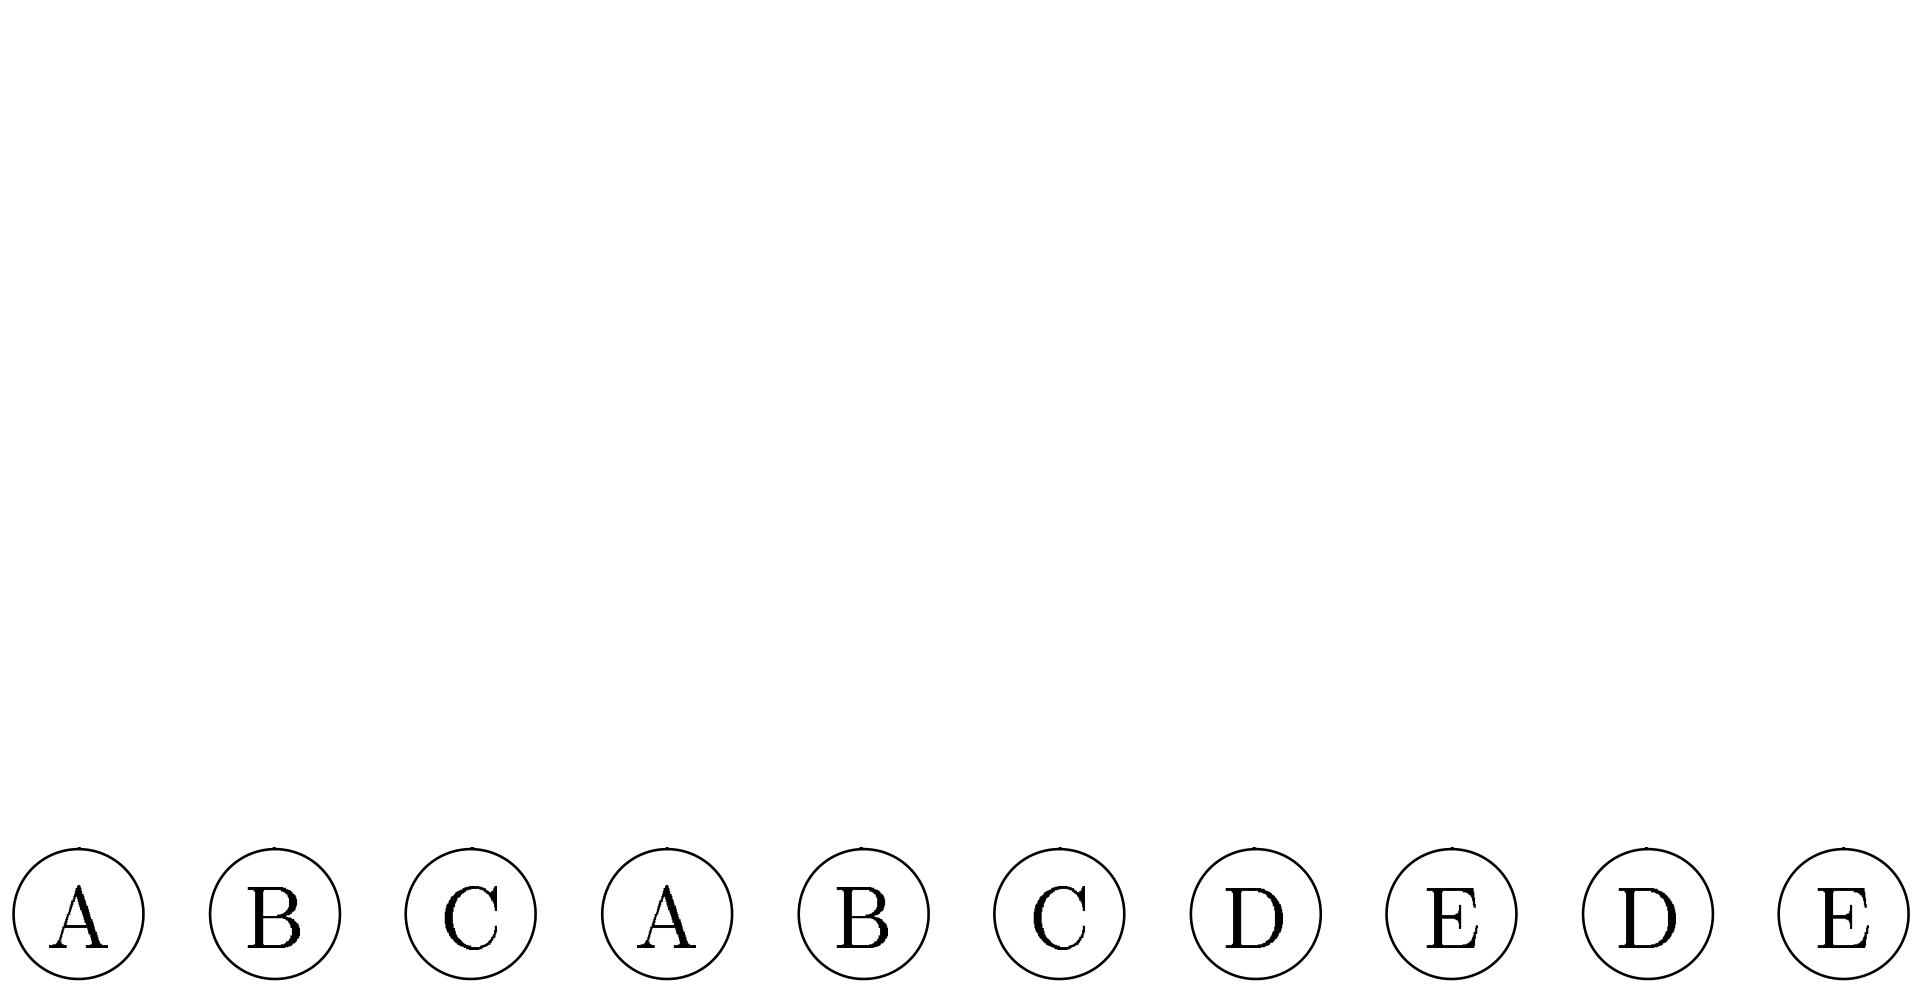
\includegraphics[scale=0.17]{creacionInc.jpg}
\end{figure}}
\pause
  \only<2>{\begin{figure}[h!]
    \centering
    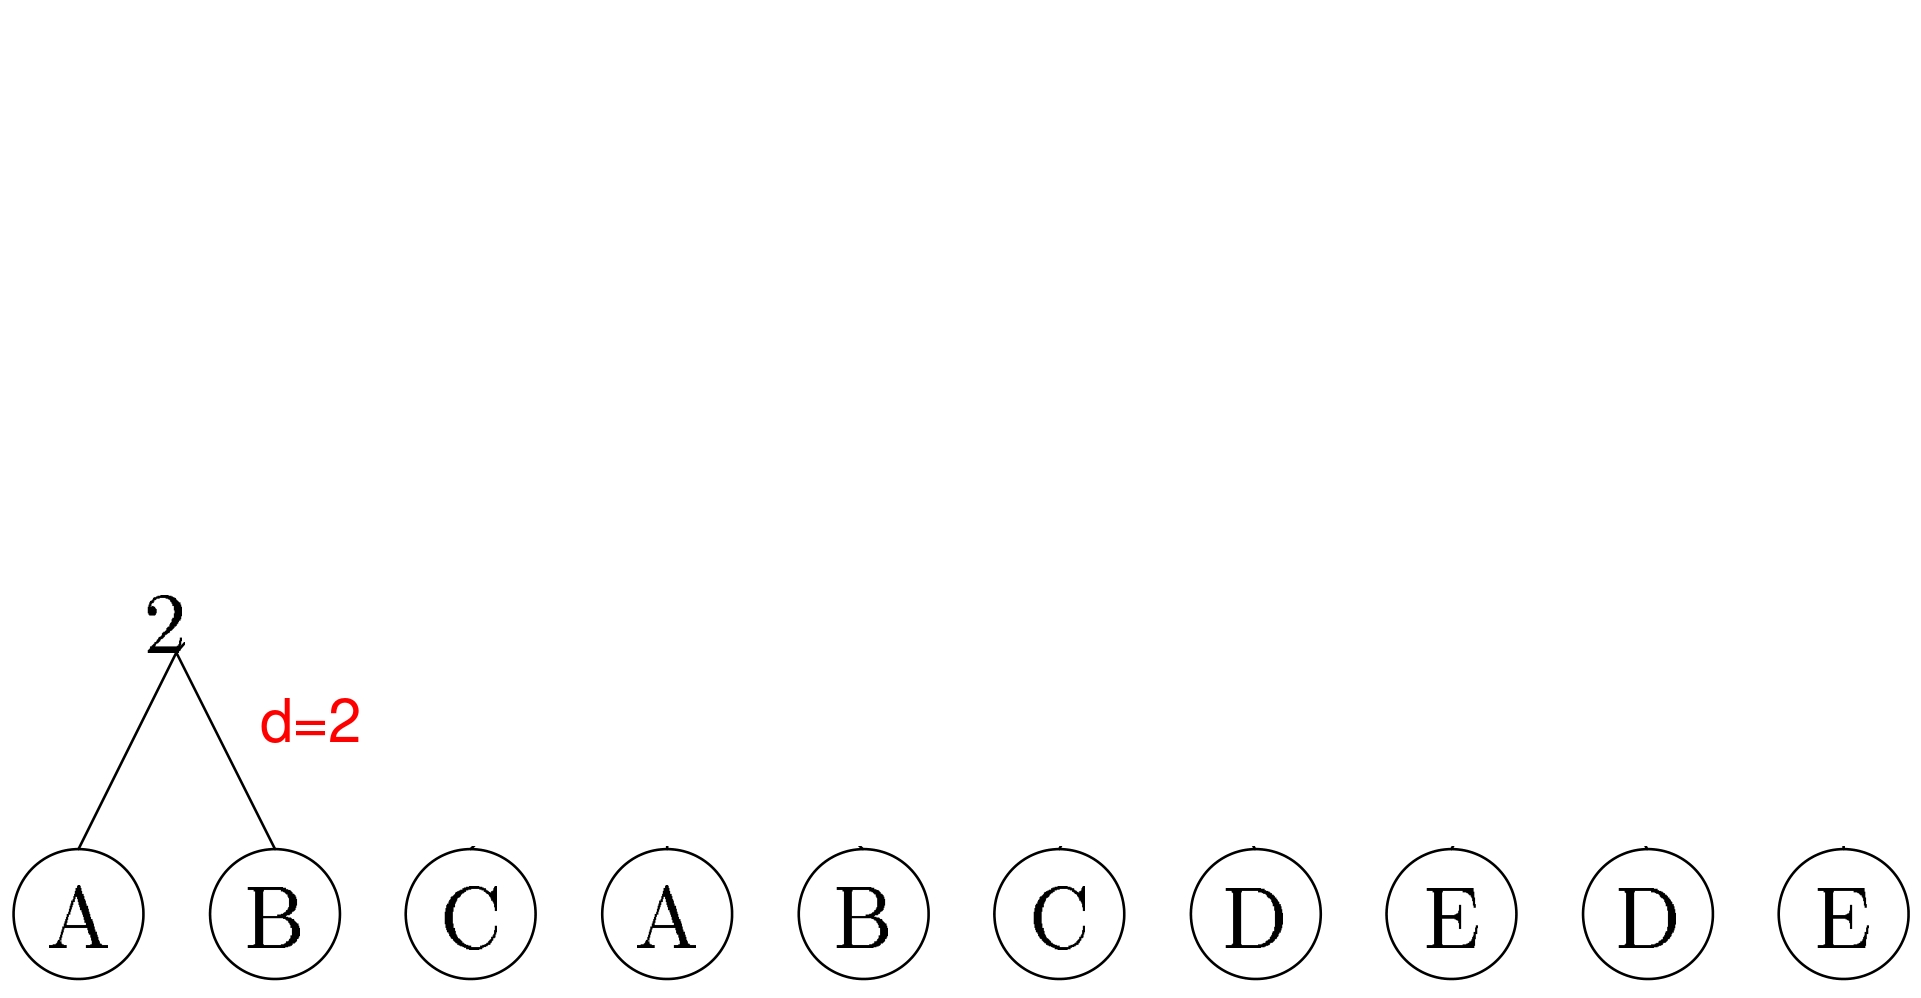
\includegraphics[scale=0.17]{creacion1.jpg}
\end{figure}}
\pause
  \only<3>{\begin{figure}[h!]
    \centering
    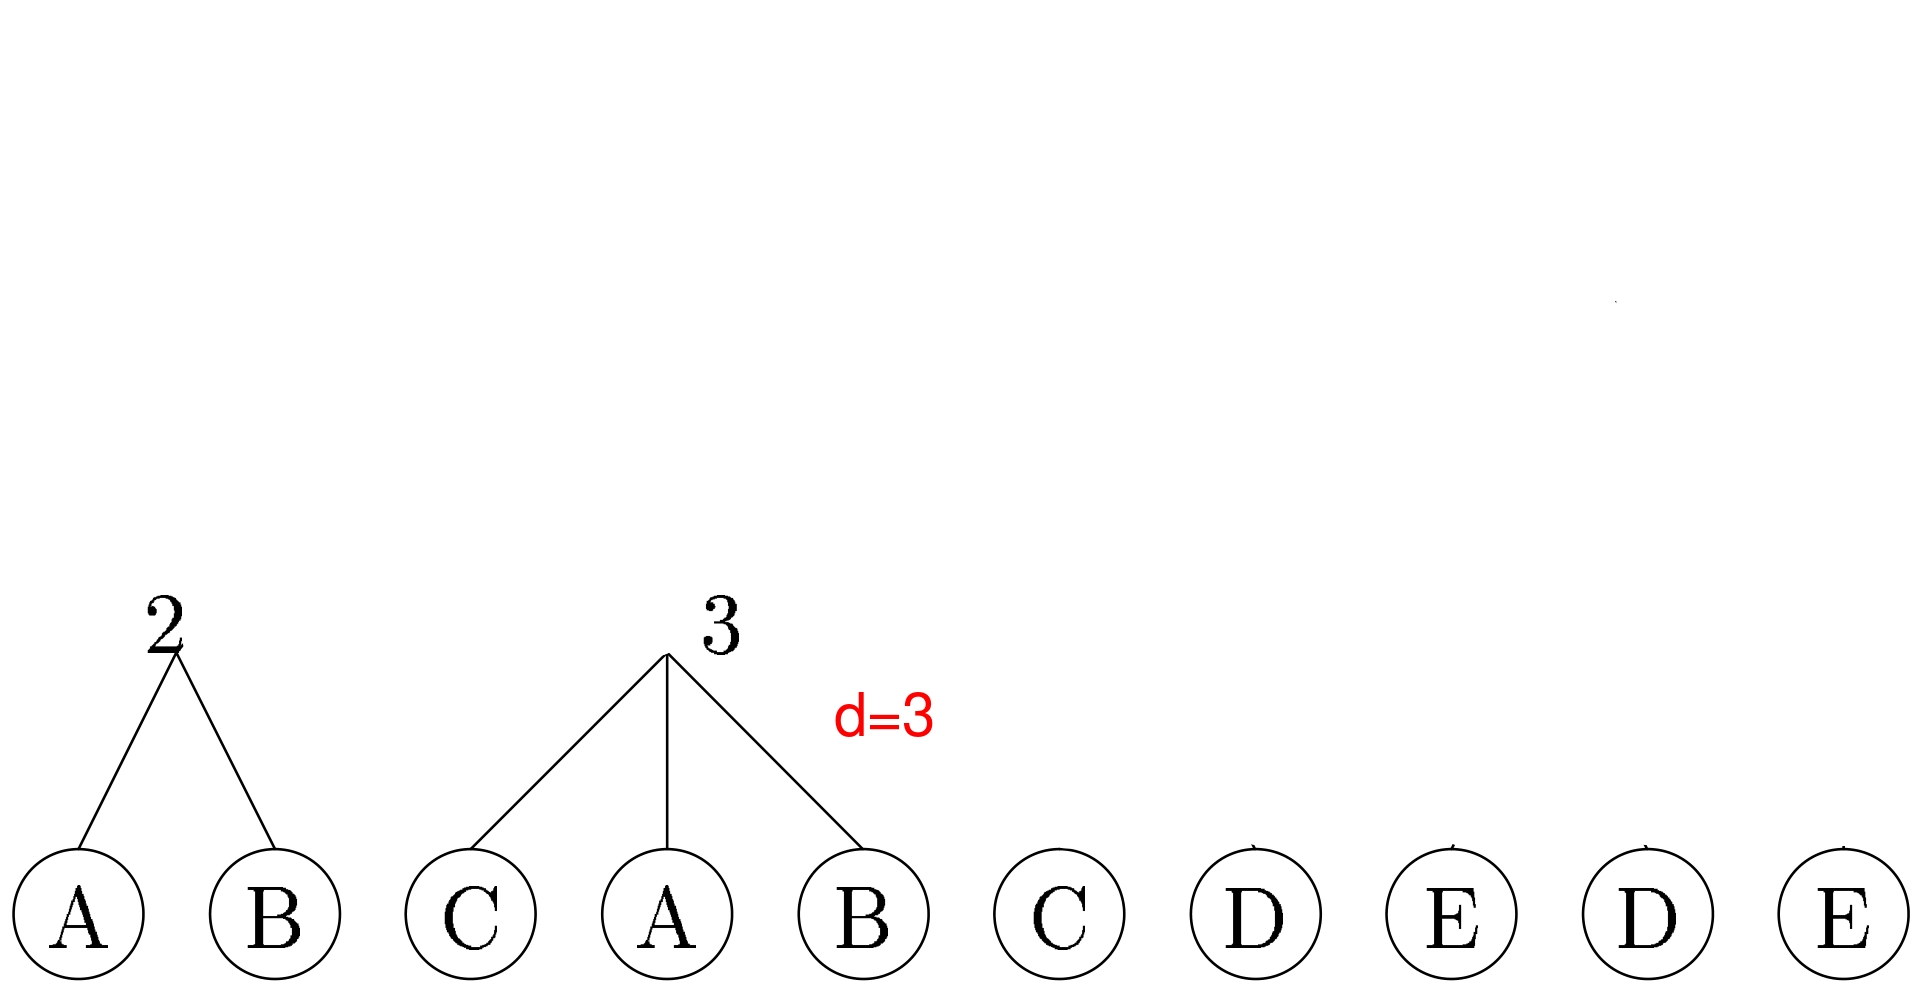
\includegraphics[scale=0.17]{creacion2.jpg}
\end{figure}}
  \pause
  \only<4>{\begin{figure}[h!]
    \centering
    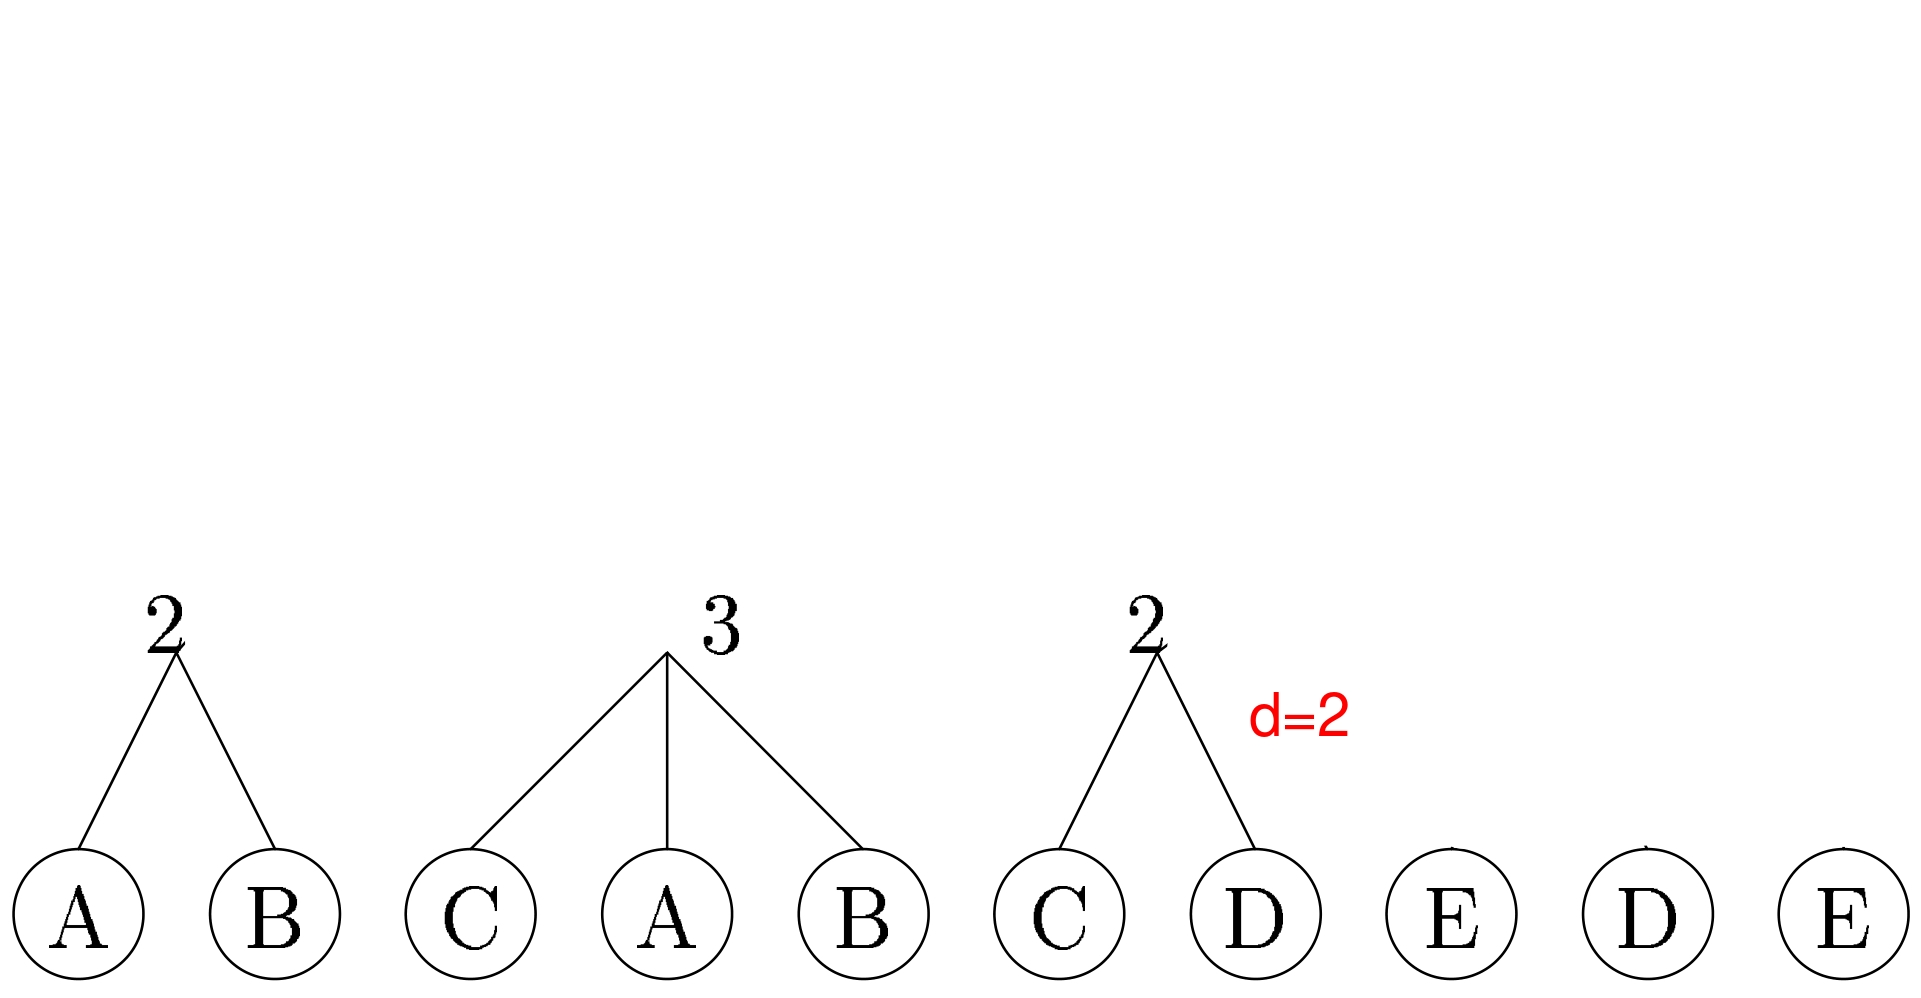
\includegraphics[scale=0.17]{creacion3.jpg}
\end{figure}}
  \pause
  \only<5>{\begin{figure}[h!]
    \centering
    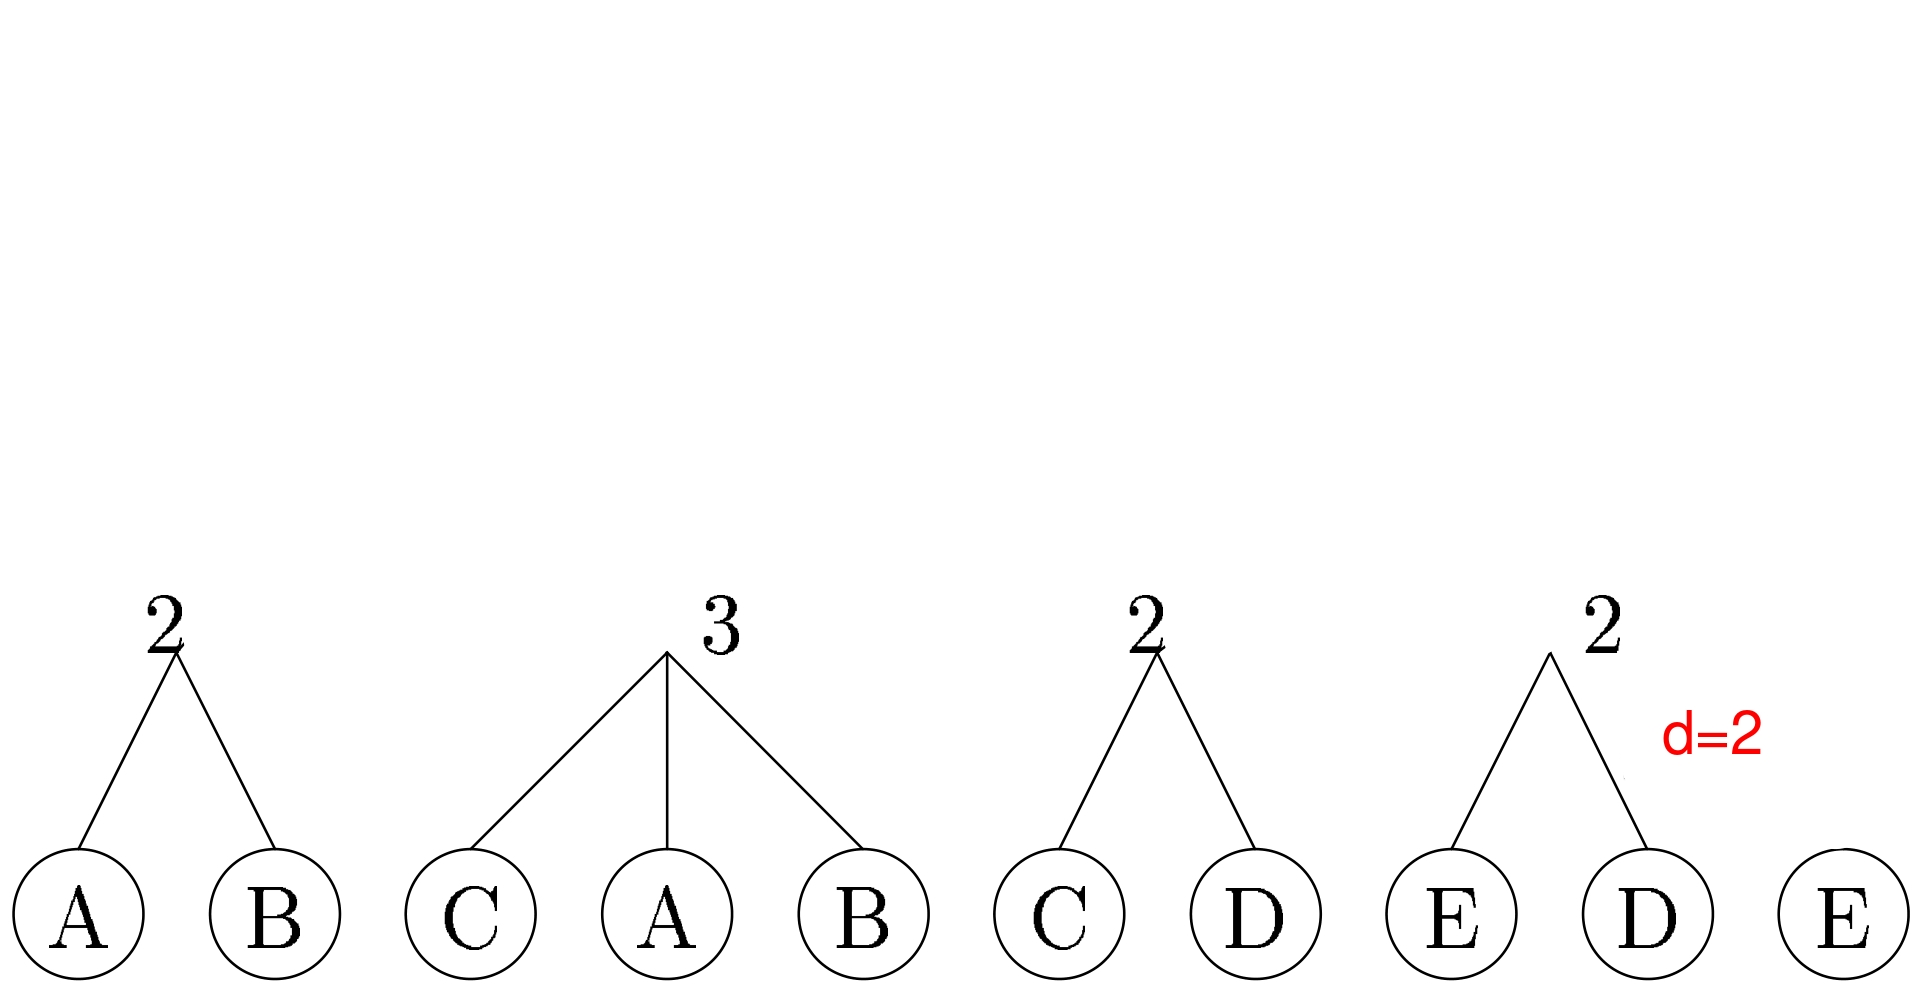
\includegraphics[scale=0.17]{creacion4.jpg}
\end{figure}}
  \pause
  \only<6>{\begin{figure}[h!]
    \centering
    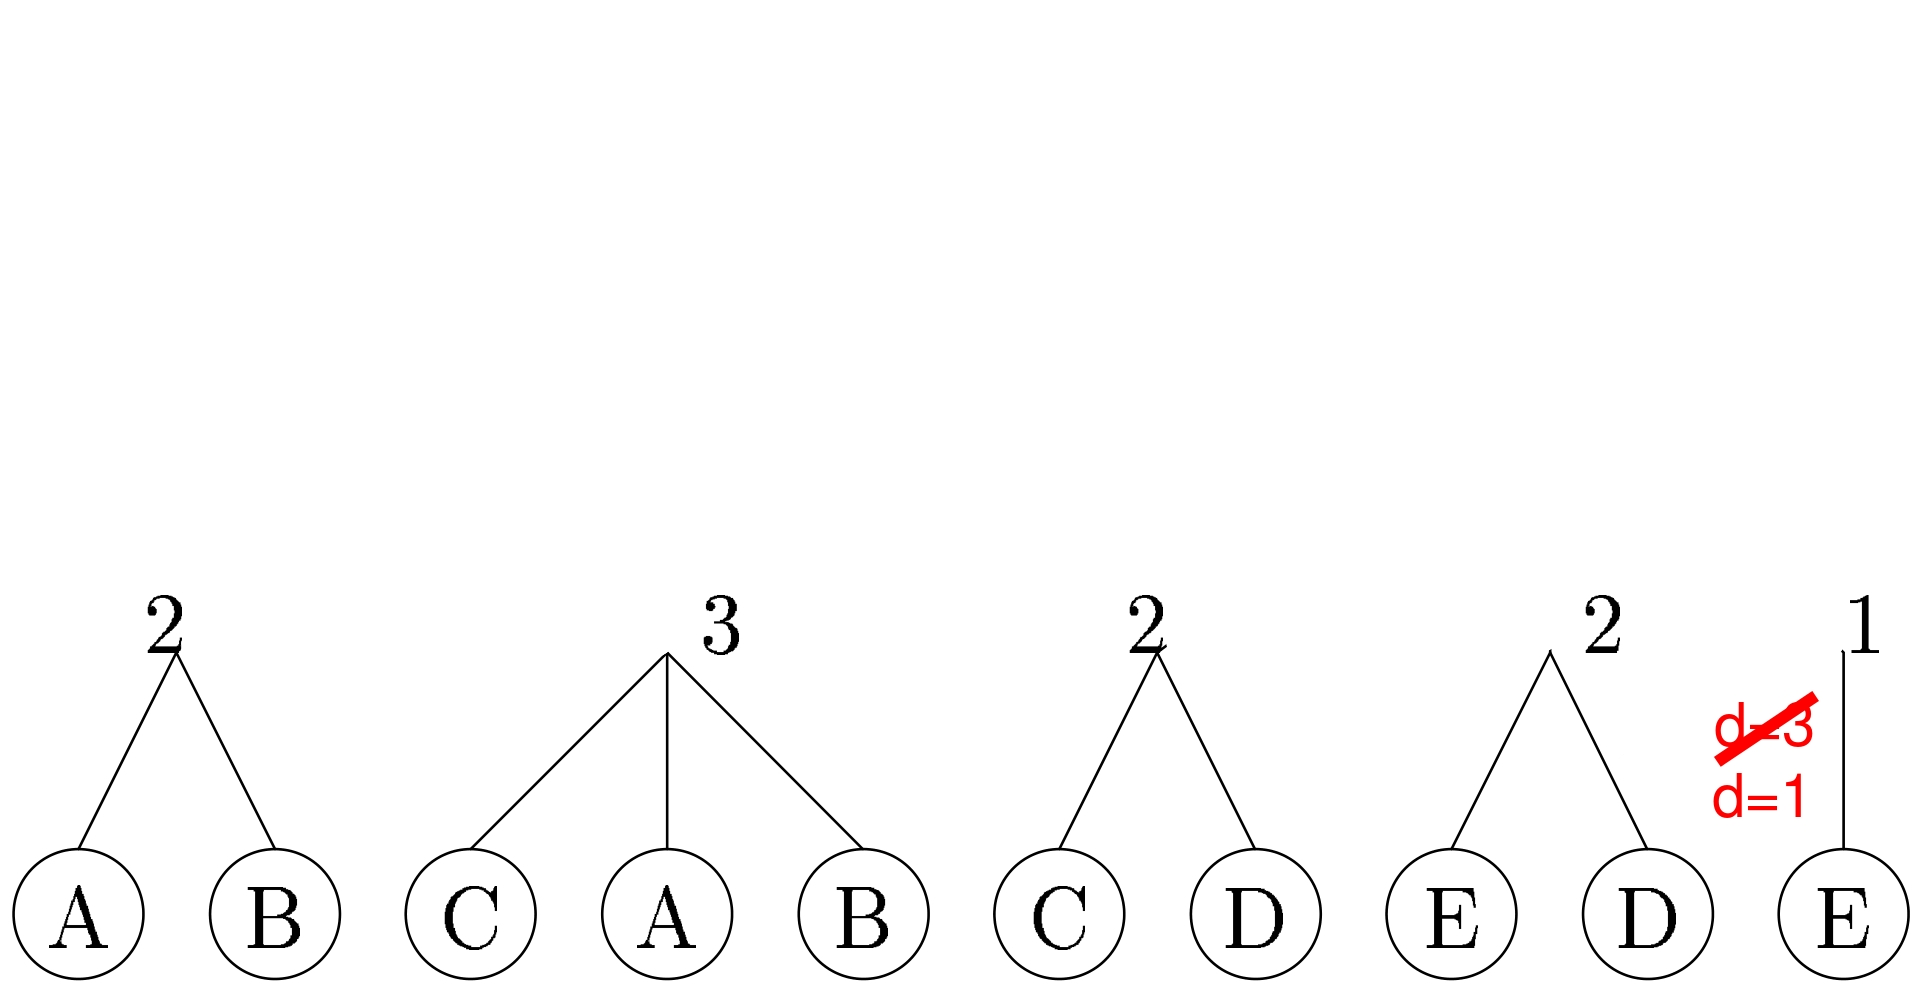
\includegraphics[scale=0.17]{creacion5.jpg}
\end{figure}}
  \pause
  \only<7>{\begin{figure}[h!]
    \centering
    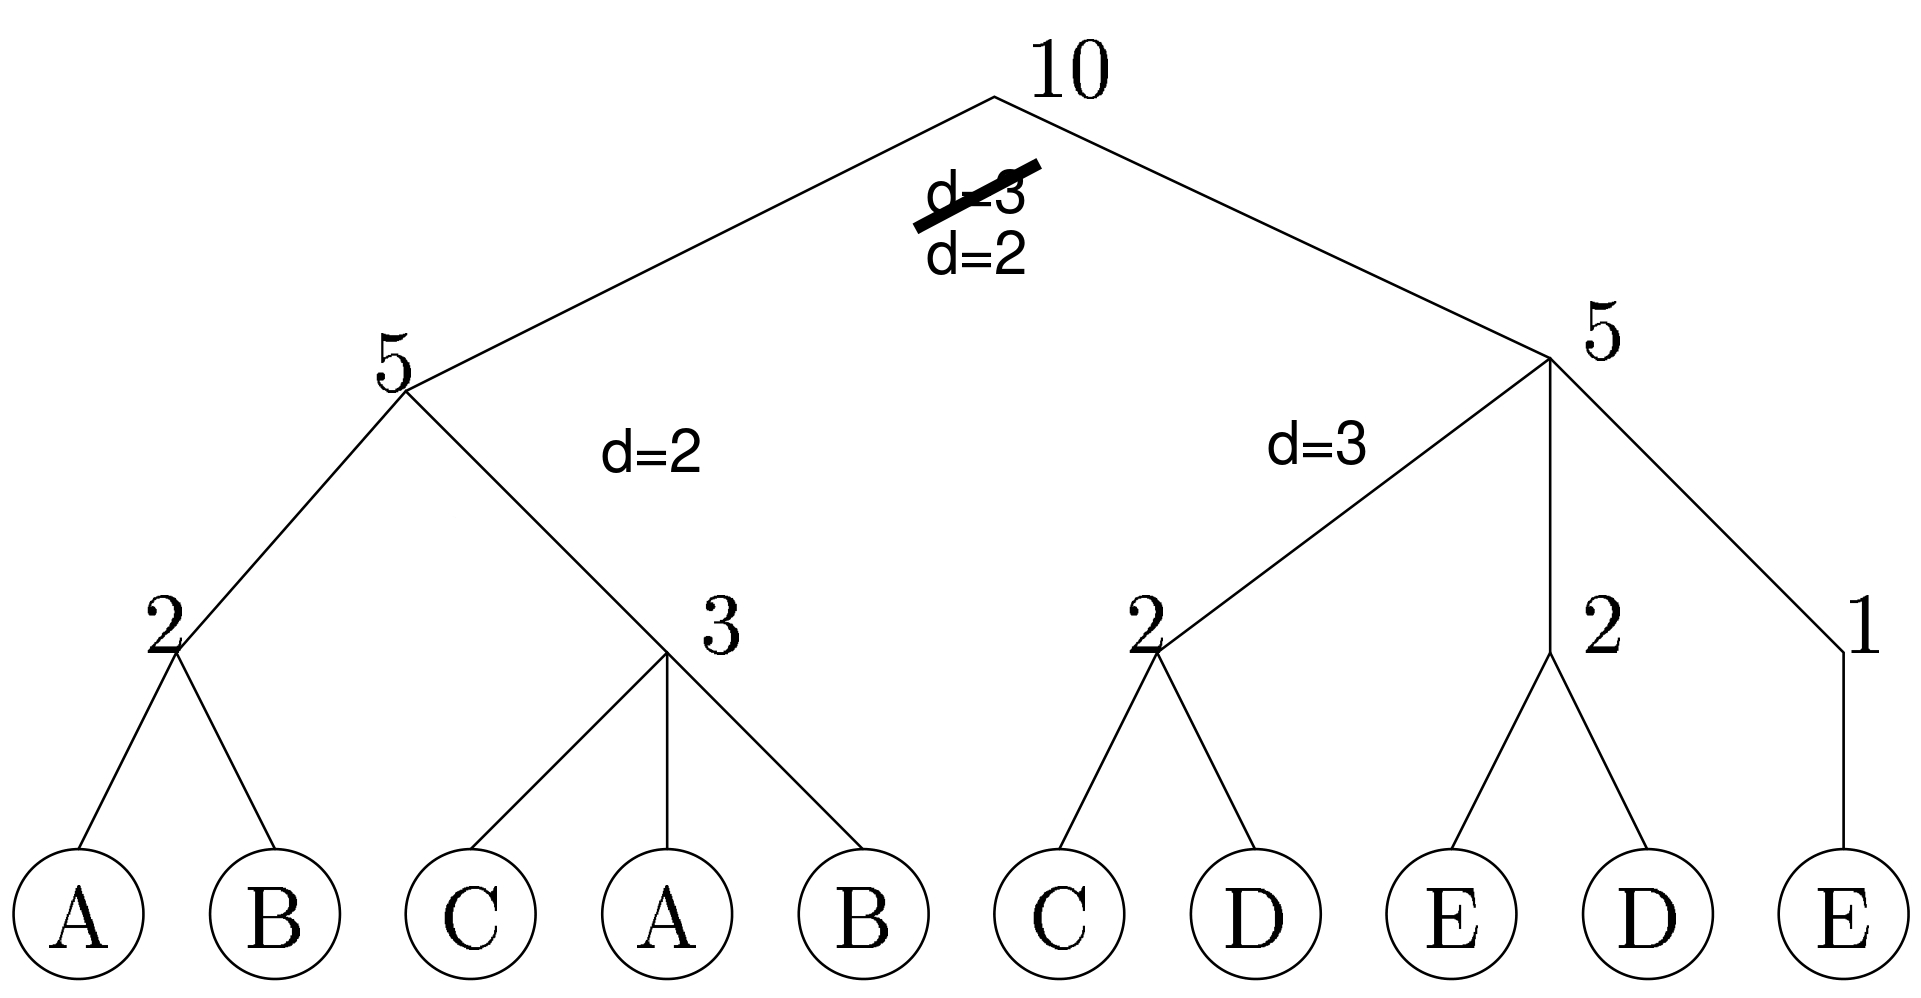
\includegraphics[scale=0.17]{creacion6.jpg}
\end{figure}}

\end{frame}

%%%%%%%%%%%%%%%%%%%%%%%%%%%%%%%%%%%%%%%%%%%%%%%%%%%%%%%%%%%%%%%%%%%%%%%%%%%%%%%%%%%%%%%%%%%%%%%%%%%%

\begin{frame}
\frametitle{Algoritmo Insertar}
  \texttt{Insertar}(i,b, T): Inserto el nodo hoja en la i-esima posición y los nodos que le siguen son agrupados
  como se hace con  \texttt{Crear} hasta que se sincroniza con el árbol.

  Son dos loops anidados.

  Tiempo: O(logn)
\end{frame}



%%%%%%%%%%%%%%%%%%%%%%%%%%%%%%%%%%%%%%%%%%%%%%%%%%%%%%%%%%%%%%%%%%%%%%%%%%%%%%%%%%%%%%%%%%%%%%%%%%%%

\begin{frame}
\frametitle{Algoritmo Insertar}
 \begin{enumerate}\itemsep-1em
  \item Inserto hoja en la i-esima posición.
  \item Loop en l: voy de l=h-1 hasta l=0.
    Donde h es la altura del árbol y $u_l$ el nodo del camino raíz a hoja en el nivel l.
\pause
    \vspace{-0.4cm}
    \begin{enumerate}[a]\itemsep-1em
    \item Si $u_l$ es el ultimo: Si $deg(u_l)=2$ listo, si $deg(u_l)=3$, se tira moneda $d$, si sale 3 listo. Recalculo los sizes.
      Si $deg(u_l)=3$ pero $d=2$ se continua al siguiente caso.
\pause
    \item Inicializo w=1 y termina con w=0 (loop en nivel l).
          \vspace{-0.4cm}
      \begin{enumerate}[i]\itemsep-1em
\pause
        \item Tiro moneda d para el grado del nodo vecino derecho a $u_l$.
        \item Transfiero los últimos w hijos de $u_l$ al vecino (si no existe lo creo).
\pause
        \item Actualizo w como w=max(0, t+w-d), donde t es el grado del nodo vecino originalmente y d lo que salio la moneda.
         \item Se re computan los tama\~nos de los nodos insertados.
      \end{enumerate}
  \end{enumerate}
\pause
  \item  Recomputa el camino desde la raíz hasta la hoja insertada.
  Si la raíz tiene nuevo vecino, creo nueva raíz.
\end{enumerate}

\end{frame}

%%%%%%%%%%%%%%%%%%%%%%%%%%%%%%%%%%%%%%%%%%%%%%%%%%%%%%%%%%%%%%%%%%%%%%%%%%%%%%%%%%%%%%%%%%%%%%%%%%%%

\begin{frame}
\frametitle{Ejemplo Insertar}
Ejemplo: \texttt{Insertar}(1, B, \texttt{Crear}(ACDE)).

  \only<1>{\centering Las dos unicas posibilidades de \texttt{Crear}(ACDE).
    \begin{figure}[h!]
    \centering
    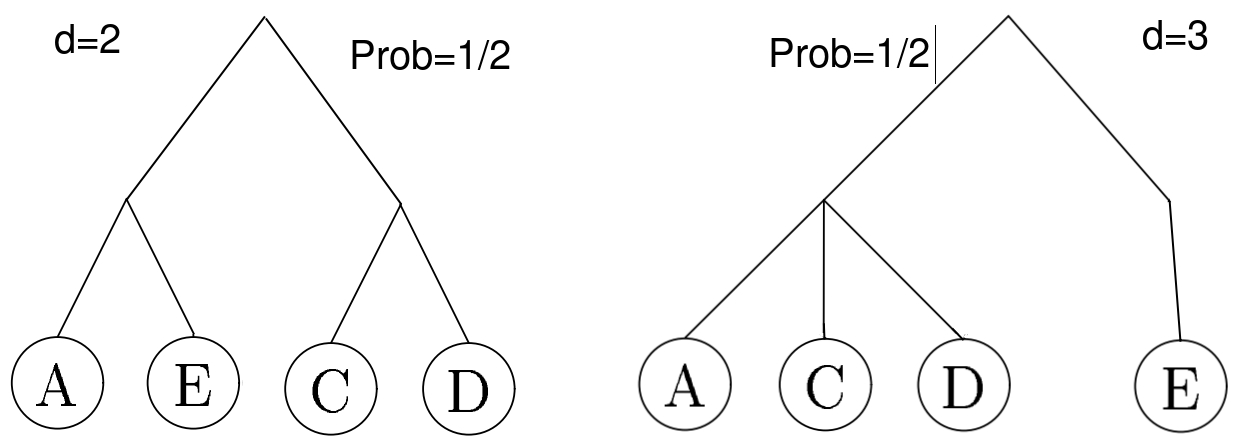
\includegraphics[scale=0.27]{insertCreate.jpg}
\end{figure}}
\pause
  \only<2>{\centering primer caso
    \begin{figure}[h!]
    \centering
    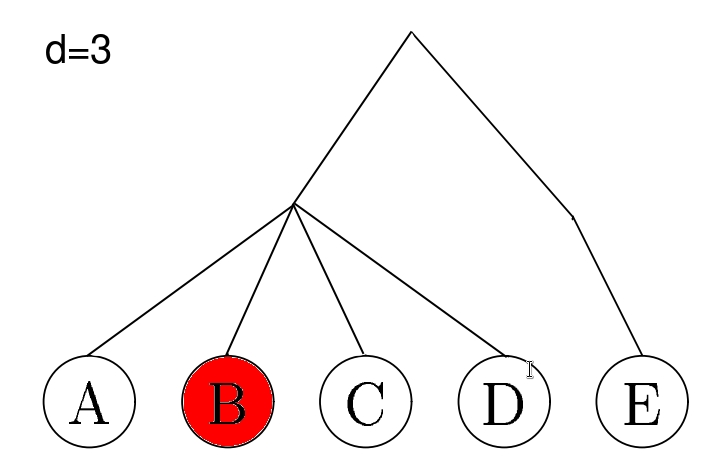
\includegraphics[scale=0.32]{insertCreateB0.jpg}
\end{figure}\centering
w=1 voy a pasarle un hijo, e independiente del d termina en 2ai/ii}
\pause
  \only<3>{\begin{figure}[h!]
    \centering
    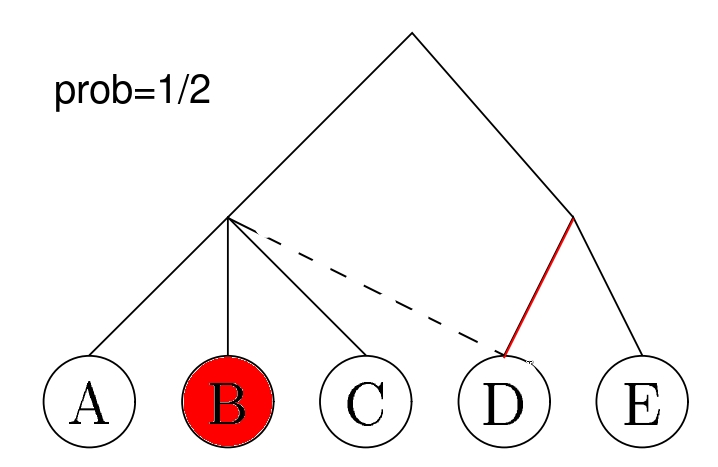
\includegraphics[scale=0.37]{insertCreateB1.jpg}
\end{figure}}
  \pause
  \only<4>{\centering segundo caso
    \begin{figure}[h!]
    \centering
    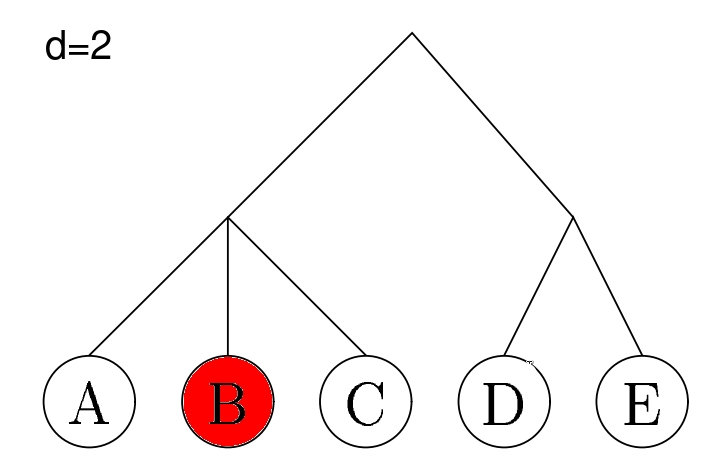
\includegraphics[scale=0.37]{insertCreateA0.jpg}
\end{figure}
\centering w=1, pasa un  hijo pero importa el d}
  \pause
  \only<5>{\centering caso d=2
    \begin{figure}[h!]
    \centering
    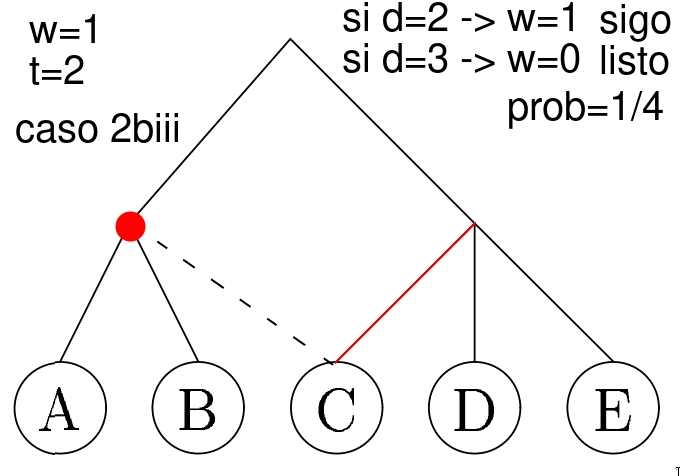
\includegraphics[scale=0.37]{insertCreateA1.jpg}
\end{figure}}
  \pause
  \only<6>{\centering caso d=2 nuevamente
   \begin{figure}[h!]
    \centering
    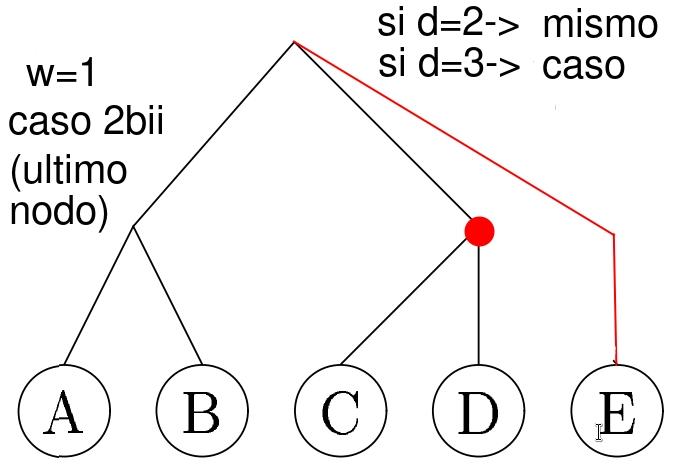
\includegraphics[scale=0.37]{insertCreateA2.jpg}
\end{figure}}
  \pause
  \only<7>{\centering Paso al nivel l-1
    \begin{figure}[h!]
    \centering
    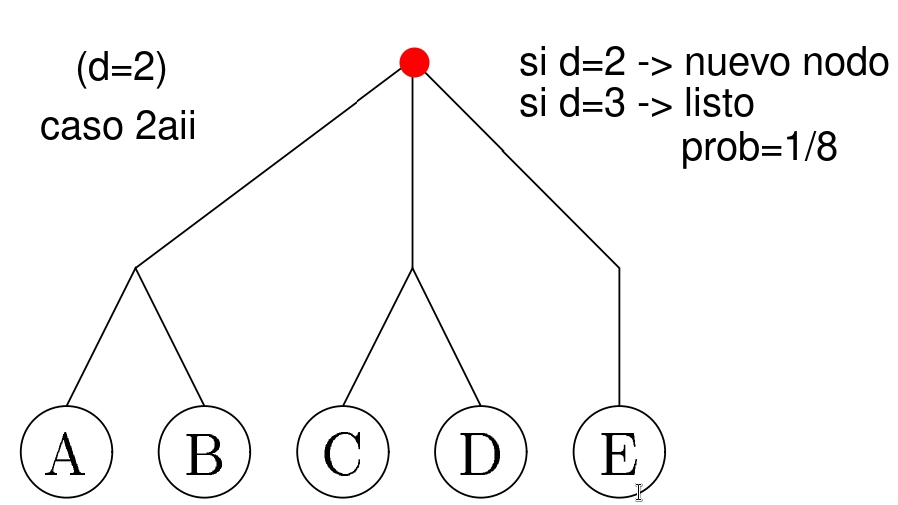
\includegraphics[scale=0.37]{insertCreateA3.jpg}
\end{figure}}
  \only<8>{\begin{figure}[h!]
    \centering
    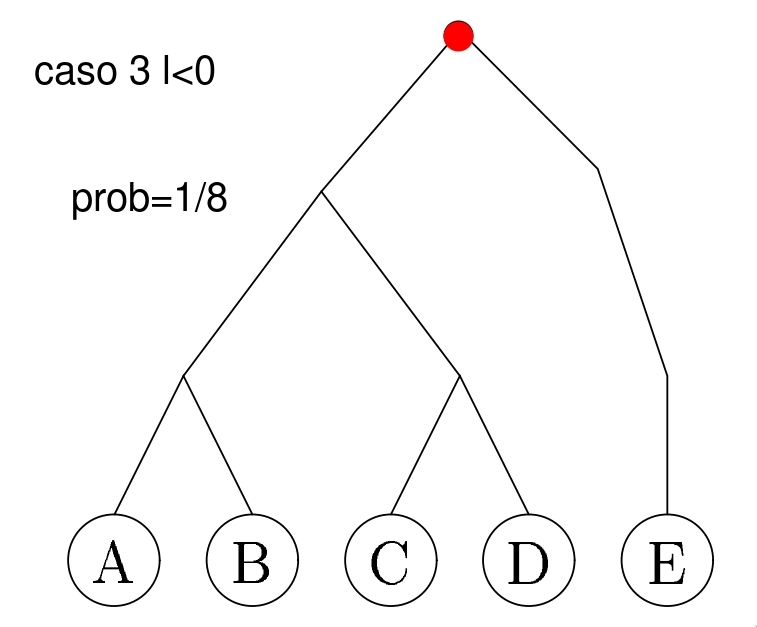
\includegraphics[scale=0.37]{insertCreateA4.jpg}
\end{figure}}



\end{frame}


%%%%%%%%%%%%%%%%%%%%%%%%%%%%%%%%%%%%%%%%%%%%%%%%%%%%%%%%%%%%%%%%%%%%%%%%%%%%%%%%%%%%%%%%%%%%%%%%%%%%

\begin{frame}
\frametitle{Borrado}
\texttt{Borrar}(i, T): Borro el nodo hoja de la i-exima posición y los nodos que le siguen son agrupados
  como se hace con  \texttt{Crear} hasta que se sincroniza con el árbol.

  Son dos loops anidados. Muy similar al Insertar, misma nomenclatura.

  Tiempo: O(logn)

\end{frame}
%%%%%%%%%%%%%%%%%%%%%%%%%%%%%%%%%%%%%%%%%%%%%%%%%%%%%%%%%%%%%%%%%%%%%%%%%%%%%%%%%%%%%%%%%%%%%%%%%%%%

\begin{frame}
\frametitle{Algoritmo Borrar}

 \begin{enumerate}\itemsep-1em
\pause
  \item Loop en l: voy de l=h-1 hasta l=0.
    Donde h es la altura del árbol y $u_l$ el nodo del camino raíz al nodo en el nivel l a remover.
    \vspace{-0.4cm}
    \begin{enumerate}[a]\itemsep-1em
    \item Borro $u_{l+1}$ de los hijos de $u_l$.
\pause
    \item Si $u_l$ es el ultimo: Si $u_{l+1}$ es el único hijo de $u_l$ paso a la siguiente iteracion, caso contrario
      voy al paso 3.
    \item Inicializo w=1 y termina con w=0 (loop en nivel l).
          \vspace{-0.4cm}
      \begin{enumerate}[i]\itemsep-1em
\pause
        \item si $w\geq t$ cambio los hijos del vecino derecho a $u_l$ y pongo w=0 y recomputo  tama\~nos.
        \item Tiro moneda d.
\pause
        \item Transfiero los  primeros w hijos del vecino derecho a $u_l$.
        \item Actualizo como w=max(0, d-t+w).
\pause
        \item Se recomputan los tama\~nos de los nodos modificados.
      \end{enumerate}
  \end{enumerate}
\pause
  \item  Recomputa el camino desde la raíz hasta la hoja insertada.
  Si la raíz tenia 2 hijos y borre 1, hago a su único hijo la raíz y borro la raíz original.
\end{enumerate}
\end{frame}
%%%%%%%%%%%%%%%%%%%%%%%%%%%%%%%%%%%%%%%%%%%%%%%%%%%%%%%%%%%%%%%%%%%%%%%%%%%%%%%%%%%%%%%%%%%%%%%%%%%%
\section{Complejidad}
\begin{frame}
\frametitle{Calculo de complejidad}

Calculo \texttt{Insertar} y \texttt{Borrar} similares.
Calculamos el primero.

Tiempo esperado  en peor caso O(logn).
\vspace{-0.2cm}
\pause


\textbf{Lema 1}: $w$ Solo toma valores \{0,1,2\}.

Rec: $w$ inicializa con 1 y si $d\neq w$ $\to$ w=max\{0, t+w-d\}.
Ademas $t\in\{1,2,3\}$ y $d\in\{2,3\}$

Dem: inducción $w\in \{0,1,2\}$

Mínimo: $t+w-d$= 1 + 1 - 3 = -1 $\rightarrow max(0, t+w-d)=0$

Máximo ($d\neq w$): t+w-d = 3+2-3= 3+1-2 = 2.


\end{frame}
%%%%%%%%%%%%%%%%%%%%%%%%%%%%%%%%%%%%%%%%%%%%%%%%%%%%%%%%%%%%%%%%%%%%%%%%%%%%%%%%%%%%%%%%%%%%%%%%%%%%
\begin{frame}
\frametitle{Calculo de complejidad}
\textbf{Lema 2}: en cada iteración del loop anidado, hay proba 1/4 de setear $w=0$ (y así terminar el loop) dentro de 2 iteraciones.
\vspace{-0.2cm}

Dem: por lema 1 sabemos que en cada iteración $w\in\{2,3\}$.
Si $u_l$ es el ultimo nodo $w=0$.
Si no, podemos tener $w=2$ y con proba 1/2 sacar d=2 y terminar.

Si tenemos $w=1$ tenemos dos casos:
\vspace{-0.3cm}
\pause
\begin{itemize}\itemsep-1em
  \item t=2: con proba 1/2 tenemos d=3 y entonces $w=t+w-d=0$, termino.
\pause
  \item t=3: con proba 1/2 tenemos d=2 y actualizamos  $w=t+w-d=2=w$, que en la siguiente
    iteración seteamos $w=0$ con probabilidad 1/2. $\to$ proba 1/4 de terminar.
\end{itemize}


\end{frame}

%%%%%%%%%%%%%%%%%%%%%%%%%%%%%%%%%%%%%%%%%%%%%%%%%%%%%%%%%%%%%%%%%%%%%%%%%%%%%%%%%%%%%%%%%%%%%%%%%%%%
\begin{frame}
\frametitle{Calculo de complejidad}



Cada nodo es visitado a lo sumo dos veces.
\begin{itemize}
  \item  O al buscar donde insertarlo y luego al recomputar su tama\~no.
  \item O al pasar por ser vecino y luego recomputar su tama\~no.
\end{itemize}


Entonces el tiempo del algoritmo será proporcional a la cantidad de nodos visitados.

Sea $T_l$ la cantidad de nodos visitados en el nivel $l$.
Tenemos dos grupos, los nodos  visitados en la iteración anidada y los nodos
visitados en el loop principal.

Sea $X_l$ la cantidad de nodos visitados en la iteración $l$.
Por el \textbf{lema 2} en cada nivel la cantidad de nodos será una distribución geométrica con parámetro 1/4 que
depende solo de las monedas tiradas en cada iteración.
Y como mucho sera dos veces.
Es decir acotado por $2X_l=2 \frac{1}{4}(1-\frac{1}{4})^x$.

\end{frame}

%%%%%%%%%%%%%%%%%%%%%%%%%%%%%%%%%%%%%%%%%%%%%%%%%%%%%%%%%%%%%%%%%%%%%%%%%%%%%%%%%%%%%%%%%%%%%%%%%%%%
\begin{frame}
\frametitle{Calculo de complejidad}

El numero de nodos visitados durante la iteración previa puede ser acotado por arriba como $T_{l+1}/2 +1$.
Ya que por propiedad del árbol 2-3 (o Oblivious) la máxima cantidad de nodos del nivel $l$ en relacion
al nivel $l+1$ es la mitad.
\begin{equation}
  Time = \sum_{i=1}^h T_i\leq \sum_{i=1}^h (T_{l+1}/2 +1 + 2X_i)
\end{equation}
paper: Si restamos de ambos lados Time/2 y multiplicamos por dos llegamos a la cota superior (?):
\begin{equation}
  Time \leq 2h + 4X
\end{equation}
Mi explicación: $T_{l+1}\leq X_i \rightarrow  Time \leq \sum_{i=1}^h (2 + 4X_i) = 2h + 4X$

Como el valor esperado de una distribución geométrica con parámetro p=1/4, es 1/p=4.

\begin{mdframed}[backgroundcolor=frenchblue!20]
  Valor esperado en peor caso: Time $\leq 2h+4(4h) \propto h=logn$
\end{mdframed}
\end{frame}

%%%%%%%%%%%%%%%%%%%%%%%%%%%%%%%%%%%%%%%%%%%%%%%%%%%%%%%%%%%%%%%%%%%%%%%%%%%%%%%%%%%%%%%%%%%%%%%%%%%%

\begin{frame}
\frametitle{Misma distribución de probabilidad.}

Queremos probar que para toda secuencia $L=L[1]L[2]...L[n]$, y sea $i\leq n$ y b una clave,
las siguientes igualdades se cumplen para las distribuciones de probabilidad.

\pause
\begin{centering}
  \texttt{Insertar}(i,b, \texttt{Crear}(L))=\texttt{Crear}(L[1],...,L[i],b,L[i+1],...,L[n])
\end{centering}

\begin{centering}
  \texttt{Borrar}(i \texttt{Crear}(L))=\texttt{Crear}(L[1],...,L[i-1],L[i+1],...,L[n])
\end{centering}

\pause
Dem: primer caso. Segundo caso análogo.

\pause
Por un lado en cada iteración $l$ solo se cambia la topología de ese nivel.
Los nodos a partir del vecino derecho en cuestion son modificados de la misma forma que \texttt{Crear} pero con
monedas diferentes e independientes.
Esto genera que tengan mismas distribuciones de probabilidad.

\end{frame}

%%%%%%%%%%%%%%%%%%%%%%%%%%%%%%%%%%%%%%%%%%%%%%%%%%%%%%%%%%%%%%%%%%%%%%%%%%%%%%%%%%%%%%%%%%%%%%%%%%%%

\begin{frame}
\frametitle{Ejemplo probabilidades}

Ejemplo con \texttt{Crear}(ABCDE) y \texttt{Insertar}(1, B, \texttt{Crear}(ACDE)).

Para el caso de insertar ya lo hicimos \texttt{Insertar} y nos dio lo siguiente:

\begin{figure}[h!]
    \centering
    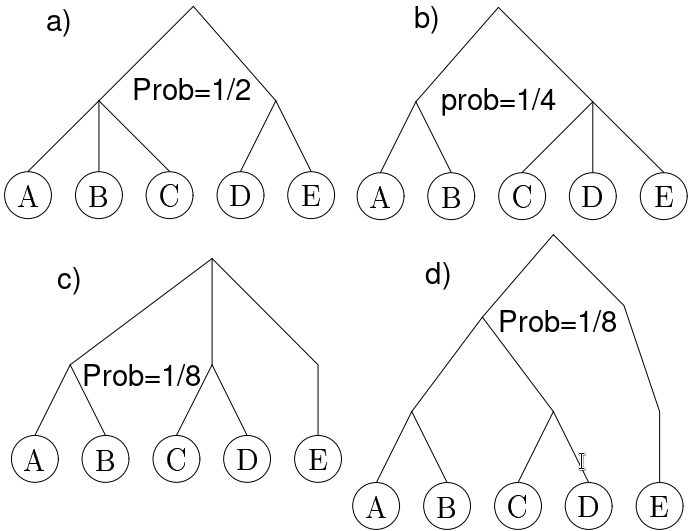
\includegraphics[scale=0.3]{insertCreateRes.jpg}
\end{figure}

\end{frame}

%%%%%%%%%%%%%%%%%%%%%%%%%%%%%%%%%%%%%%%%%%%%%%%%%%%%%%%%%%%%%%%%%%%%%%%%%%%%%%%%%%%%%%%%%%%%%%%%%%%%

\begin{frame}
\frametitle{Ejemplo probabilidades}

Basta con probar que \texttt{Crear}(ABCDE) tiene las mismas probabilidades.

\begin{itemize}
  \item Primer caso, d=3 prob 1/2, termina (caso a). \pause
  \item Segundo caso d=2, prob 1/2, sigue en el siguiente nodo:
\pause
    \begin{itemize}\pause
      \item d=3, con prob 1/2*1/2=1/4, termina (caso b).\pause
      \item d=2, prob 1/2*1/2=1/4, termina en ese nivel pero sigue en el próximo:
\pause
        \begin{itemize}\pause
          \item d=3, prob 1/4*1/2=1/8, termina (caso c).\pause
          \item d=2, prob 1/4*1/2=1/8, crea un nodo al lado de la raíz. Se crea
            un nuevo nivel con nueva raíz.
        \end{itemize}
    \end{itemize}
\end{itemize}

\pause

Comprobado!

\end{frame}
%%%%%%%%%%%%%%%%%%%%%%%%%%%%%%%%%%%%%%%%%%%%%%%%%%%%%%%%%%%%%%%%%%%%%%%%%%%%%%%%%%%%%%%%%%%%%%%%%%%%

\section{Conclusiones}
\begin{frame}
\frametitle{Conclusiones}
\begin{itemize}
  \item Árbol de búsqueda balanceado aleatorio.
  \item Algoritmos de edición en O(logn).
  \item Permite privacidad sin costo extra.
\end{itemize}
\begin{figure}[h!]
    \centering
    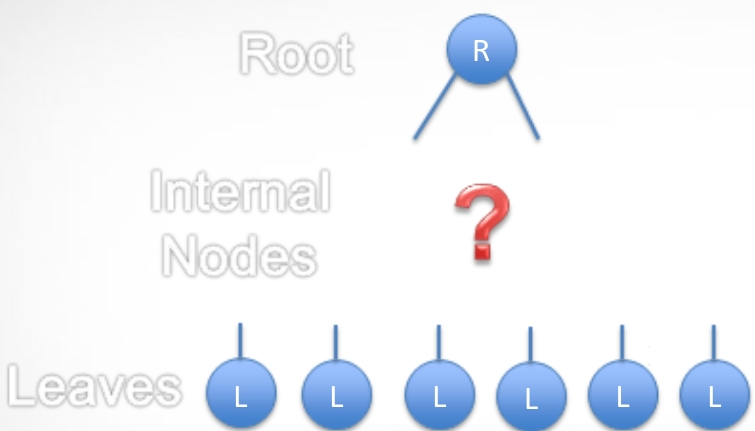
\includegraphics[scale=0.3]{conc.jpg}
\end{figure}


\end{frame}


%%%%%%%%%%%%%%%%%%%%%%%%%%%%%%%%%%%%%%%%%%%%%%%%%%%%%%%%%%%%%%%%%%%%%%%%%%%%%%%%%%%%%%%%%%%%%%%%%%%%

\section{}
\begin{frame}
\frametitle{}

\huge
\centering
FIN!
\end{frame}

%%%%%%%%%%%%%%%%%%%%%%%%%%%%%%%%%%%%%%%%%%%%%%%%%%%%%%%%%%%%%%%%%%%%%%%%%%%%%%%%%%%%%%%%%%%%%%%%%%%%

\section{}
\begin{frame}[noframenumbering]
  \frametitle{Algoritmo insertar completo}
\small
\begin{enumerate}\itemsep0em
  \item Localizo la i-esima hoja e inserto el valor. Sea $u_0,...,u_h$ el camino
    de la raiz a la nueva hoja.
  \item Repetimos los siguientes pasos de l=h-1,h-2,...,0. Donde en cada iteracion
    es de la raiz al nuevo nodo.
    \vspace{-0.05cm}
    \begin{enumerate}[a]\itemsep0em
      \item Si $u_l$ es el ultimo nodo del nivel l:
        \vspace{-0.05cm}
        \begin{enumerate}[i]\itemsep0em
          \item Si $u_l$ tiene grado 2 entonces ir al paso 3.
          \item Si $u_l$ tiene grado 3, elijo de forma uniforme $d\in{2,3}$ y si
            $d=4$ ir al paso 3, si no continuar.
        \end{enumerate}
      \item Inicializamos la variable w=1 y repetimos los pasos hasta w=0:
        \vspace{-0.05cm}
        \begin{enumerate}[i]\itemsep0em
          \item Sea $u_l'=u_l$ y elegimos de forma uniforme $d\in{2,3}$. d es el grado
            del nodo que sigue a $u_l'$.
          \item Si d=w o si $u_l'$ es el ultimo nodo al nivel l, insertamos el nuevo nodo $u_l$
            a la derecha de $u_l'$, seteamos w=0 y vamos al paso 2(b)v.
          \item En caso contrario, hacemos $u_l$ el nodo que continua a $u_l'$ en el nivel l y
            sea t=deg($u_l$) (el que tenia de antes).
          \item Cambiamos de padre los ultimos $w$ hijos de $u_l'$ a $u_l$ y hacemos $w=max(0, t+w-d)$.
          \item Recomputamos el tama\~no de los nodos a lo largo del camino de $u_l'$ a $u_l$ no incluido.
        \end{enumerate}
    \end{enumerate}
  \item Si $l\geq$0, recomputamos la informacion de tama/~no de los nodos del camino.
    En caso contrario aumentamos la altura del arbol en uno creando un nuevo nodo raiz
    y hacemos de hijos $u_0'$ y el nuevo nodo $u_0$
\end{enumerate}

\end{frame}
%%%%%%%%%%%%%%%%%%%%%%%%%%%%%%%%%%%%%%%%%%%%%%%%%%%%%%%%%%%%%%%%%%%%%%%%%%%%%%%%%%%%%%%%%%%%%%%%%%%%

\section{}
\begin{frame}[noframenumbering]
\frametitle{Algoritmo borrar completo}
\small
\begin{enumerate}\itemsep0em
  \item Localizo la i-esima hoja e inserto el valor. Sea $u_0,...,u_h$ el camino
    de la raiz a la nueva hoja.
  \item Repetimos los siguientes pasos de l=h-1,h-2,...,0. Donde en cada iteracion
    es de la raiz al nuevo nodo.
    \vspace{-0.05cm}
    \begin{enumerate}[a]\itemsep0em
      \item Si $u_l$ es el ultimo nodo del nivel l:
        \vspace{-0.05cm}
      \item Borramos $u_{l+1}$ de los hijos de $u_l$.
      \item Si $u_l$ es el ultimo nodo del nivel: Si $u_{l+1}$ era el unico hijo de $u_l$
      , continuamos con la siguiente iteracion del loop 2, si no al paso 3.
      \item Inicializamos la variable w=1 y repetimos los pasos hasta w=0:
        \vspace{-0.05cm}
        \begin{enumerate}[i]\itemsep0em
          \item Sea $u_l'=u_l$ y movemos para adelante $u_l$.
          \item Hacemos t=deg($u_l$). Si $w\geq t$, cambiamos los paodres de los hijos de $u_l$
            a $u_l'$, seteamos w=0 y vamos al paso 2(c)v.
          \item Elegimos de forma uniforme $d\in{2,3}$.
          \item Cambiamos de padre los primeros $w$ hijos de $u_l'$ a $u_l$ y hacemos $w=d-t+w)$.
          \item Recomputamos el tama\~no de los nodos a lo largo del camino de $u_l'$ a $u_l$ no incluido.
        \end{enumerate}
    \end{enumerate}
  \item Si $l\geq$0, recomputamos la informacion de tama/~no de los nodos del camino.
    En caso contrario borramos el nodo $u_0$ y hacemos $u_1$ la nueva raiz del arbol.
\end{enumerate}

\end{frame}
%%%%%%%%%%%%%%%%%%%%%%%%%%%%%%%%%%%%%%%%%%%%%%%%%%%%%%%%%%%%%%%%%%%%%%%%%%%%%%%%%%%%%%%%%%%%%%%%%%%%


\section{}
\begin{frame}[noframenumbering]
\frametitle{B-tree}
Un mero repaso:

\begin{columns}
    \column{0.5\textwidth}
    Árbol auto balanceado de búsqueda.
    \begin{itemize}
\pause
       \item Balanceado: Permite búsquedas en peor caso de O(long).
       \item Búsqueda: Mantiene orden dentro del árbol.
\pause
       \item Utilización: Reducir accesos al disco, (arboles grandes que no entran en memoria principal).
       \item Arboles B de grado M
    \end{itemize}

    \column{0.5\textwidth}
    Árbol B de grado M.
        \begin{itemize}
\pause
          \item Cada noto tiene como Máximo M hijos.
          \item Un nodo que no sea hoja con k hijos contiene k-1 claves.
          \item La raíz tiene como mínimo 2 hijos a menos que sea hoja.
\pause
          \item Todo nodo que no sea ni raíz ni hoja tiene al menos M/2 hijos.
          \item Todas las hojas están al mismo nivel.
          \item Las claves están ordenadas en cada nodo.
        \end{itemize}
\end{columns}
\end{frame}
%%%%%%%%%%%%%%%%%%%%%%%%%%%%%%%%%%%%%%%%%%%%%%%%%%%%%%%%%%%%%%%%%%%%%%%%%%%%%%%%%%%%%%%%%%%%%%%%%%%%


\end{document}

